\documentclass[11pt,a4paper]{article}
\usepackage[show]{ed}
\usepackage{tikz}
\usepackage{float}
\usepackage{hyperref}
\usepackage[style=alphabetic, backend=bibtex]{biblatex}
\usepackage{graphicx}

\title{Building MathHub using React\\ \vspace{2 mm} Bachelor Thesis}
\author{Johannes-Sebastian See\\Supervisor: Michael Kohlhase\\Co-supervisor: Tom Wiesing\\Friedrich-Alexander University, Erlangen Nürnberg, Germany}

\date{\today}
\addbibresource{local.bib}

\providecommand\myxscale{.95}
\providecommand\myyscale{1}

\begin{document}

\begin{titlepage}
\maketitle
\begin{abstract}
Abstract will be added at the end
\end{abstract}

\end{titlepage}

\tableofcontents
\section{Introduction}
\subsection{Math Information Systems}
\ednote{why are those special and different}
\ednote{System to impart mathematical knowledge to people}
\begin{itemize}
\item Zentral Blatt Math
\item mlfdb
\item Wolfram alpha
\item isu-afp.org
\item mathoverflow: Q{\&}A site for mathematicians to discuss unsolved math problems
\item Wikidata: central storage for Wikimedia
\item Wikipedia: part of Wikimedia
\item what can they do? what is their goal? what can we do different/better?
\end{itemize}
\subsection{MathHub}
\subsection{Previous Implementation}
Up until April 2018 the MathHub frontend was realized with Drupal.
Drupal is an open source content-management framework used by millions of different websites.
User interactions were handled by JavaScript modules in the JOBAD framework \cite{comp}.
	
But in April 2018 a critical security flaw in the versions 6 to 8 went public.
The problem was that Drupal in these versions accepts request parameters without any validation.
This means it processes any input from anybody \cite{zdnet}.
To exploit this weakness an attacker doesn't even need to log in or have any other privileges on a vulnerable website \cite{register}.
With this flaw it is possible to inject malicious code and compromise a website in multiple ways.
This can be used to access, change and delete private data and create backdoors to make future attacks possible.
The Drupal community called this weakness "Drupalgeddon2" while its official name was "CVE-2018-7600".
Some code that was injected installed the program XMRig Monero miner, which is a cryptocurrency mining program, as well as deleting other mining programs on the compromised system \cite{hacker}.
The National Institute of Standards (NIST) and Technology gave Drupal a "Highly Critical" Rating because of this vulnerability \cite{nist}.
 After this flaw was discovered a patch was published and a warning to update every website that used a vulnerable version was given.
	
Since there have been multiple flaws in Drupal before that compromised MathHub.info, the decision to stop using it and rebuild MathHub.info from the ground up to not be affected by future attacks, was made. \ednote{This is too much detail. Shorten this}

\vspace{4cm} \noindent
This thesis describes the individual parts of building the new MathHub.info.
It starts with some frameworks that can be used to create a frontend in section \ref{SoA}.
Following up on this, section \ref{react} and \ref{components} takes a closer look at React while \ref{mmt} gives a short introduction to the content of MathHub.
Then section \ref{architecture} is about the inner workings of the frontend.
Afterwards in section \ref{library} and \ref{apps} the design of the individual pages are discussed.
At the end of this thesis the conclusion can be found in section \ref{conclusion} and some plans for the future in section \ref{future}.

\section{State of the art - Building an interactive Frontend} \label{SoA}
Before starting to build a completely new MathHub frontend a new web framework had to be chosen.

\textbf{Polymer} \cite{polymer} is an open source JavaScript library developed and maintained by Google.
It uses the native technologies of a browser instead of large custom JavaScript libraries.
This makes Polymer remarkably fast on Chrome and Safari.
It also provides a set of features that makes it easy to create custom elements, that work like standard web components.
It is used for several Google services for example Youtube, Google Earth, Google Play Music etc. as well as Netflix, Electronic Arts and many other companies. 

Another open source web framework from Google is \textbf{Angular}. \cite{angular}
This TypeScript library has framework architectures that simplifies the development of new web applications.
Angular transfers all content of a website at once and leaves the task of building the page to the browser.
This significantly speeds up the loading process and search optimization while keeping the communication with the server at a minimum. 
It also has Angular Material.
A collection of UI components that work in browsers, on mobile and desktop.

After using Angular on several Google projects, Evan You decided to create his own JavaScript framework called \textbf{Vue.js} \cite{vuewiki}
Depending on the project it can be scaled between a framework and a library.
Vue.js separates its view layer library from its support libraries for complex applications, to create an easy approach to the framework.
It also automatically keeps track of the dependencies between components.
So the system knows what exactly has to be rerendered when the page changed.\cite{vuegit}

In the end the decision was made to use \textbf{React} developed by Facebook.
React is a component based framework that uses a virtual DOM to avoid unnecessary rerendering.
It was chosen because the focus on reusable components makes it perfect for a large and still growing system like MathHub.\ednote{@Tom: Is this why we chose it???}
Further details about React and how it is used can be found in section \ref{preliminaries}.


\section{Preliminaries} \label{preliminaries}
\subsection{The core concept of React} \label{react}
React is an open source JavaScript library owned and maintained by Facebook.
It was created to build interactive user interfaces (UI), for example Facebook and Instagram.
What makes React unique is its use of a virtual Document Object Model (DOM).
The concept of the virtual DOM is that updating a website does not rerender everything.
React computes the differences between the last and the next page and only changes the necessary parts.
On top of that it also has conditional rendering which means that an item will only be rendered if it is shown.
The advantage of the virtual DOM and conditional rendering is that this makes updating a website fast, but it comes with high RAM costs.
The actual interface is made up of many different elements and components.
A website that uses React can have multiple unique features so it is helpful to build new components to realize these features.\cite{reactjs}
Further detail are discussed in section \ref{components}.

Since React was designed by Facebook, there was a need for a design pattern that handles a large code base better than MVC (Model View Controller).
That is why Flux was created.
The philosophy of the Flux design is that data flows only in one direction to create unidirectional cycles. \cite{flux}

React does not have a styling system so its community created the Semantic UI React library to provide an easy way to maintain a consistent theme throughout the frontend.
Of course it is still possible to use a different library or create new styling components but MathHub.info mostly uses Semantic UI React.

\subsection{Building new components in React} \label{components}
The actual interface that can be seen in a browser is the combination of many individual components.
This way, on an update, the virtual DOM can check each component for differences, so only the affected ones have to be rendered again.

React already has a large external library with a lot of different components, but it is often necessary to make new ones that have a desired functionality.
In JavaScript new components can either be implemented as a function or as a class.
Their inputs are called props.
To ensure the unidirectional design of React props are read-only.
In addition to props components can have an internal state.
They return React elements that are ready to be rendered.
Naturally a component can grow big rather quickly.
Luckily it is possible to use components inside other components.
As a consequence, the actual output often has a tree structure with several levels.
Where the nodes of the tree are the individual components and the leaves are the elements that are rendered by the DOM.
Figure \ref{fig:tree} displays one possible tree with four levels.
This design comes with the advantage that the small components can be reused in many different locations with various purposes.

\begin{figure}[H]
\centerline{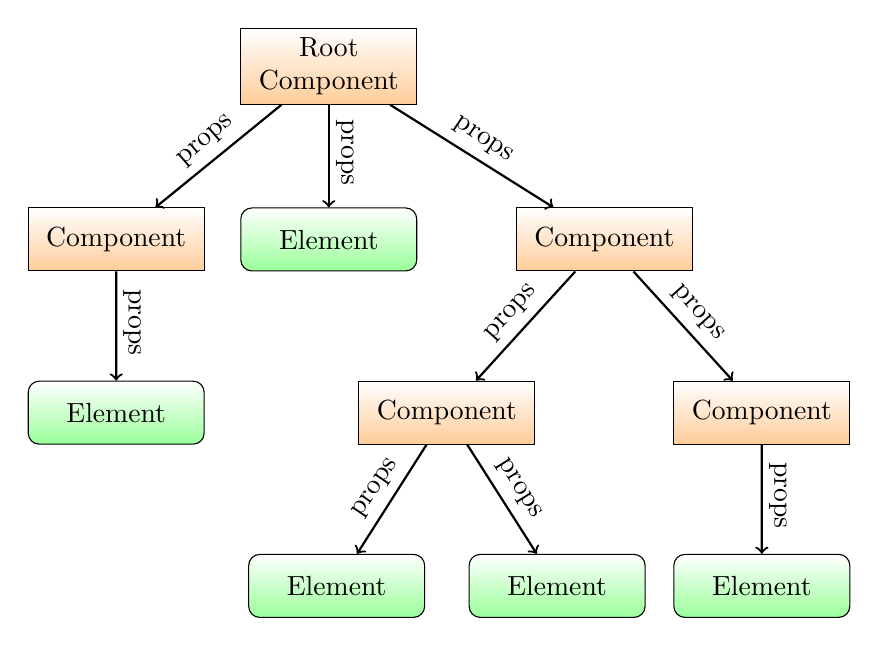
\begin{tikzpicture}[xscale=\myxscale, yscale=\myyscale]
  \tikzstyle{node} = [rectangle, draw, fill=orange!20, text width=2cm, yshift=-1.2cm, text centered,
                                    minimum height=.8cm,shade, 
                                    top color=white, bottom color=orange!40]
  \tikzstyle{leave} = [rectangle, draw, fill=green!20, text width=2cm, text centered, yshift=-1.2cm,
                                    rounded corners, minimum height=.8cm,shade, 
                                    top color=white, bottom color=green!40]
\node[node](root){Root Component};
\node[node, below of=root, xshift=-2.7cm](com1){Component};
\node[leave, below of=root](elem1){Element};
\node[node, below of=root, xshift=3.5cm](com2){Component};
\node[leave, below of=com1](elem2){Element};
\node[node, below of=com2, xshift=-2cm](com3){Component};
\node[node, below of=com2, xshift=2cm](com4){Component};
\node[leave, below of=com3, xshift=-1.4cm](elem3){Element};
\node[leave, below of=com3, xshift=1.4cm](elem4){Element};
\node[leave, below of=com4](elem5){Element};
\draw[->, thick] (root) -- node[above, rotate=41]{props} (com1);
\draw[->, thick] (root) -- node[right, xshift=0.2cm, yshift=0.6cm, rotate=270]{props} (elem1);
\draw[->, thick] (root) -- node[above, rotate=326]{props} (com2);
\draw[->, thick] (com1) -- node[right, xshift=0.2cm, yshift=0.6cm, rotate=270]{props} (elem2);
\draw[->, thick] (com2) -- node[above, rotate=48]{props} (com3);
\draw[->, thick] (com2) -- node[above, rotate=312]{props} (com4);
\draw[->, thick] (com3) -- node[above, rotate=56]{props} (elem3);
\draw[->, thick] (com3) -- node[above, rotate=302]{props} (elem4);
\draw[->, thick] (com4) -- node[right, xshift=0.2cm, yshift=0.6cm, rotate=270]{props} (elem5);
\end{tikzpicture}}
\caption{A React component tree}
\label{fig:tree}
\end{figure}
                            
Since props are read-only, updating the internal state of a component can only affect its children.
If it is necessary to change something in a component on a higher level in the tree, it is possible to "lift up" the state.
This means adding the change to the state of the higher node. 
This node then has to give it back to its child as a prop.

Sometimes an update of a state should affect other components on the same level.
As shown in figure \ref{fig:lift}, this can be done by lifting up the state to a new node in the tree that has all the components as children, that are affected by the update.
\cite{reactjsGS}
 
\begin{figure}[H]
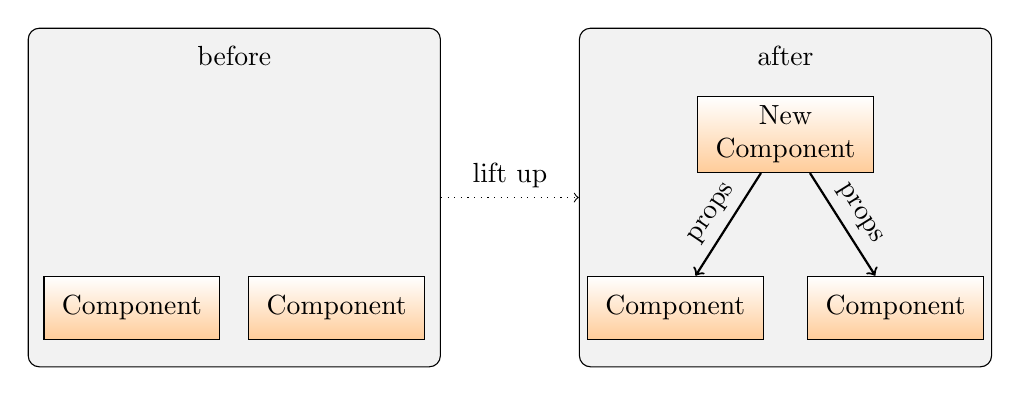
\begin{tikzpicture}[xscale=\myxscale, yscale=\myyscale]
  \tikzstyle{node} = [rectangle, draw, fill=orange!20, text width=2cm, text centered,
                                    minimum height=.8cm,shade, 
                                    top color=white, bottom color=orange!40]
                                    top color=white, bottom color=green!40]
  \tikzstyle{back} = [rectangle, draw, fill=gray!10, text width=5cm,
                                    rounded corners, minimum height=4.3cm]
\node[back, label ={[shift={(0ex,-4ex)}]north:before}](oldb){};
\node[node, below of=oldb, xshift=-1.3cm, yshift=-0.4cm](com1){Component};
\node[node, right of=com1, xshift=1.6cm](com2){Component};
\node[back, right of=oldb, xshift=6cm, label ={[shift={(0ex,-4ex)}]north:after}](newb){};
\node[node, below of=newb, yshift=1.8cm](new){New Component};
\node[node, below of=new, xshift=-1.4cm, yshift=-1.2cm](com3){Component};
\node[node, below of=new, xshift=1.4cm, yshift=-1.2cm](com4){Component};
\draw[->, thick] (new) -- node[above, rotate=56]{props} (com3);
\draw[->, thick] (new) -- node[above, rotate=302]{props} (com4);
\draw[->, dotted] (oldb) -- node[above]{lift up} (newb);
\end{tikzpicture}
\caption{Lift up the state to a new component}
\label{fig:lift}
\end{figure}

\subsection{MMT and OMDoc} \label{mmt}
The abbreviation MMT is short for either \underline{m}eta-\underline{m}eta-\underline{t}heory or \underline{m}eta-\underline{m}eta-\underline{t}ool.
Whereby meta-meta-theory represents the theoretical and meta-meta-tool the practical part of MMT.
It is a knowledge representation framework that uses a combination of formal and informal languages to create a scalable module system for mathematical theories.
That means that in MMT the features of the syntax and the semantics of a language are defined as individual, reusable modules.
This way of building individual languages leads to a high degree of abstraction of advanced algorithms.\cite{mmtsys}

MMT builds on the OMDoc representation, which is a philosophy about the design of an uniform language for knowledge.
More specifically MMT uses an XML fomat which follows this philosophy.

\begin{figure}[H]
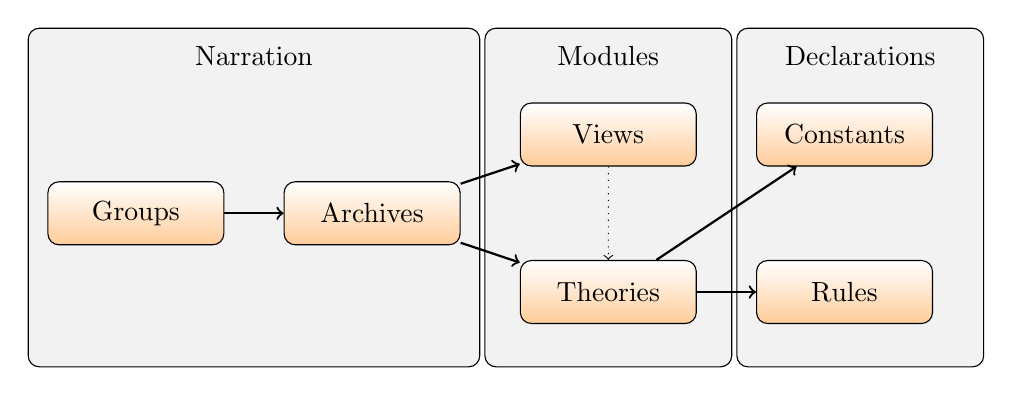
\begin{tikzpicture}[xscale=\myxscale, yscale=\myyscale]
  \tikzstyle{component} = [rectangle, draw, fill=orange!20, text width=2cm, text centered,
                                    rounded corners, minimum height=.8cm,shade, 
                                    top color=white, bottom color=orange!40]
  \tikzstyle{back} = [rectangle, draw, fill=gray!10, text width=2cm,
                                    rounded corners, minimum height=4.3cm]
\node[back, text width = 5.5cm,  label ={[shift={(0ex,-4ex)}]north:Narration}] (nar) {};
\node[back, right of =nar, xshift=3.5cm, text width = 2.9cm,  label ={[shift={(0ex,-4ex)}]north:Modules}] (mod) {};
\node[back, right of =mod, xshift=2.2cm, text width = 2.9cm,  label ={[shift={(0ex,-4ex)}]north:Declarations}] (dec) {};
\node[component, left of =nar, xshift=-0.5cm, yshift=-0.2cm] (groups) {Groups};
\node[component, right of =groups, xshift=2cm] (archives) {Archives};
\node[component, right of =archives, xshift=2cm, yshift=-1cm] (theo) {Theories};
\node[component, right of =archives, xshift=2cm, yshift=1cm] (views) {Views};
\node[component, right of=theo, xshift=2cm, yshift=2cm] (con) {Constants};
\node[component, right of=theo, xshift=2cm] (rul) {Rules};
\draw[->, thick] (groups) -- node[above]{} (archives);
\draw[->,thick] (archives) -- node[above]{} (theo);
\draw[->,thick] (archives) -- node[above]{} (views);
\draw[->,thick] (theo) -- node[above]{} (rul);
\draw[->,thick] (theo) -- node[above]{} (con);
\draw[->,dotted] (views) -- node[above]{} (theo);
\end{tikzpicture}
\caption{The MMT structure}
\label{fig:mmt}
\end{figure}


To create a frontend that displays MMT it is important to understand its structure, that can be seen in figure \ref{fig:mmt}.
First up on the highest level are the individual groups.
Each group contains several archives.
An archive can be described as a collection of documents that typically are equivalent to a software project.
So it provides a work flow for a language in MMT.
Groups and archives only exist for navigation and narration purposes.
The modules that can be found in an archive, make up the actual content.
These are either a theory or a view that shows the relation between different theories.
A theory is defined by its rules and constants, the so called declarations.
\cite{mmt}
 
\section{The Architecture of MathHub} \label{architecture}

\subsection{MathHub.info Routes}
\begin{figure}[H]
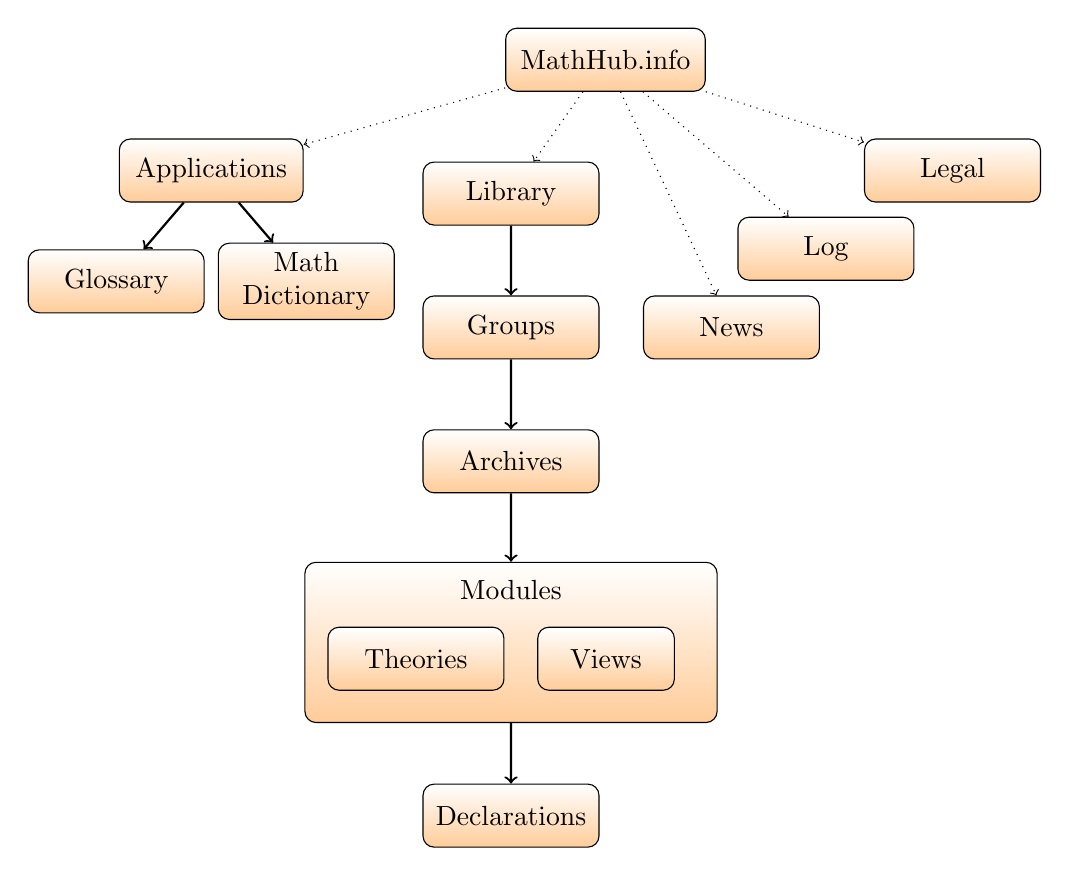
\begin{tikzpicture}[xscale=\myxscale, yscale=\myyscale]
  \tikzstyle{component} = [rectangle, draw, fill=orange!20, text width=2cm, text centered,
                                    rounded corners, minimum height=.8cm,shade, 
                                    top color=white, bottom color=orange!40]
                                   
\node[component, text width=2.3cm] (MH) {MathHub.info};
\node[component, below of =MH, xshift=-1.2cm, yshift=-0.7cm] (lib) {Library};
\node[component, below of =lib, yshift=-0.7cm] (groups) {Groups};
\node[component, below of =groups, yshift=-0.7cm] (archives) {Archives};
\node[component, below of =archives, text width=5cm, text height=1.8cm, yshift=-1.3cm, label ={[shift={(0ex,-4ex)}]north:Modules}] (mod) {};
\node[component, below left of =mod, xshift=-0.5cm, yshift=0.5cm] (theo) {Theories};
\node[component, below right of =mod, text width=1.5cm, xshift=0.5cm, yshift=0.5cm] (views) {Views};
\node[component, below of=mod, yshift=-1.2cm] (decl) {Declarations};
\node[component, below left of =MH, xshift = -4.3cm, yshift=-0.7cm, text width=2.1cm] (apps) {Applications};
\node[component, below left of =apps, xshift=-0.5cm, yshift=-0.7cm] (glos) {Glossary};
\node[component, below right of =apps, xshift=0.5cm, yshift=-0.7cm] (dict) {Math Dictionary};
\node[component, below of=MH, xshift=1.6cm, yshift=-2.4cm] (news) {News};
\node[component, below of=MH, xshift=2.8cm, yshift=-1.4cm] (log) {Log};
\node[component, below right of=MH, xshift=3.7cm, yshift=-0.7cm] (legal) {Legal};
\draw[->,dotted] (MH) -- node[above]{} (lib);
\draw[->,dotted] (MH) -- node[above]{} (apps);
\draw[->,dotted] (MH) -- node[above]{} (news);
\draw[->,dotted] (MH) -- node[above]{} (log);
\draw[->,dotted] (MH) -- node[above]{} (legal);
\draw[->,thick] (lib) -- node[above]{} (groups);
\draw[->, thick] (groups) -- node[above]{} (archives);
\draw[->,thick] (archives) -- node[above]{} (mod);
\draw [->,thick] (mod) -- node[above]{} (decl);
\draw[->,thick] (apps) -- node[above]{} (glos);
\draw[->,thick] (apps) -- node[above]{} (dict);
\end{tikzpicture}
\caption{MathHub routes}
\label{fig:routes}
\end{figure}


To create a logical navigation system MathHub.info uses routes to divide its content into numerous pages, that can be accessed from the Homepage.
The structure of these routes can be seen in figure \ref{fig:routes}.

First of is the main content of MathHub, the MMT library.
It starts with the different groups.
The next page displays the archives that belong to a specific group.
Groups and archives exist only for narration and navigation purposes.
So they don't have any actual content only meta information like names and descriptions.
The actual content can be found in documents.
These document consist of multiple modules (i.e. theories and views) as well as opaque elements that give the user additional information about the theories.
So the archive-page has a list of all the documents in an archive.
On the document-page the modules are displayed with all their declarations.

With the huge mathematical library of theories there are a lot of technical terms.
The glossary is a collection of these expressions.
There wouldn't be much value in to just having a collection without any additional features.
So the glossary also provides a definition for each term.
Over the time many different authors have contributed to the theories, so it can happen that there are different terms that share a meaning.
These synonyms can also be found in the glossary.
Since many theories exist in multiple languages it makes sense to have a glossary available for every used language.
Currently the biggest collection of terms are in the English glossary, followed by German and French.
Smaller collections for Turkish and Romanian are also available as well as simplified and traditional Chinese.\cite{smglom}

Most of the times a user does not want to browse through the gigantic glossary to just find a single term.
This is the reason why the Math Dictionary is a useful extension of the glossary.
The main purpose of the Math Dictionary is to translate a term into another language and look up a definition of a specific expression.

There is also a page with all the latest news regarding MathHub, as well as a couple of static pages like licenses and privacy policy.
At last there is a Log with the most recent messages from the backend.

\subsection{Layout}
Every page consists of three parts: A header, a footer and the actual content in between.
This is illustrated with the Homepage as an example in figure \ref{fig:home}.

\begin{figure}[H]
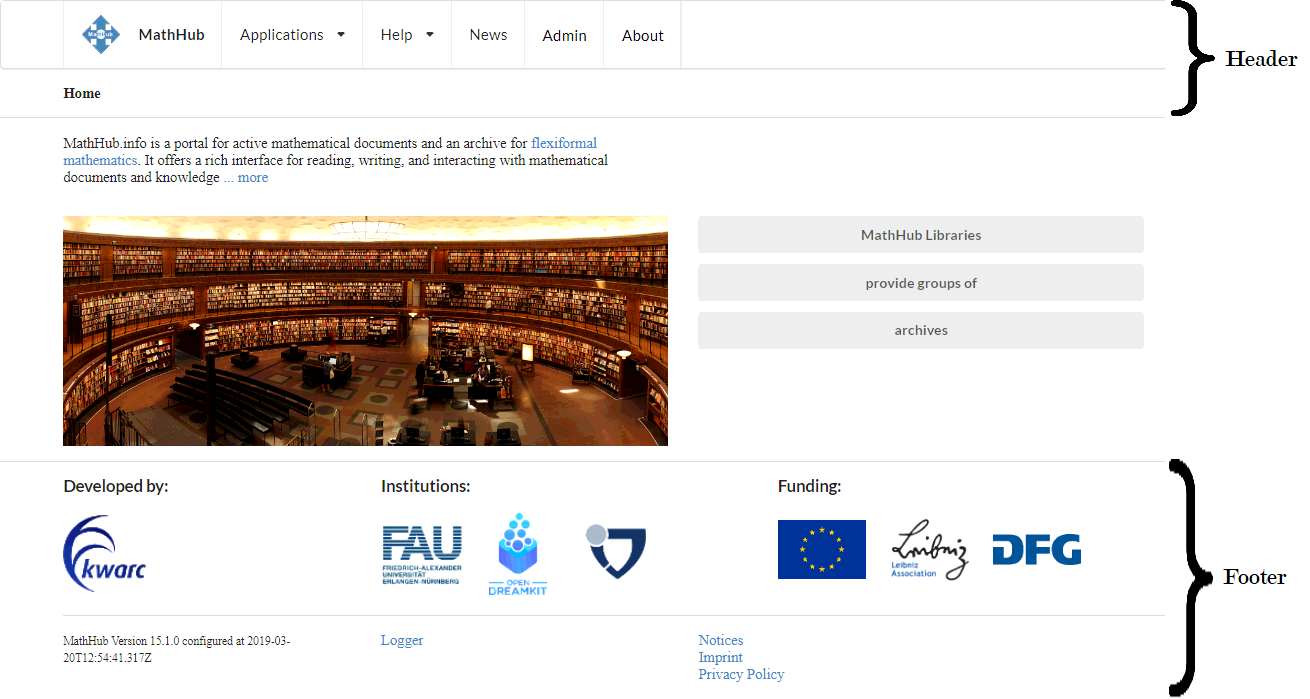
\includegraphics[width=1\textwidth]{home2.png}
\caption{The Homepage}
\label{fig:home}
\end{figure}

The header is a menu with the routes to Home, the news, the glossary and the Math Dictionary as well some external links.
Under the menu there are breadcrumbs for an easier navigation.
In the footer the logos of the institutions that are involved in MathHub can be found.
There also are the routes to the Log, the licenses, the imprint and the privacy policy.
The body itself depends on the page the user is currently on.

\subsection{Realization}
\ednote{name pending}
\begin{figure}[H]
\begin{tikzpicture}[xscale=\myxscale,yscale=\myyscale]
  \tikzstyle{system} = [rectangle, draw, fill=orange!20, text width=1cm, text centered,
                                    rounded corners, minimum height=.8cm,shade, 
                                    top color=white, bottom color=orange!20]
   \tikzstyle{database} = [rectangle, draw, fill=blue!20, text width=1.3cm, text centered,
                                    rounded corners, minimum height=.8cm,shade, 
                                    top color=white, bottom color=blue!20] 
\node[inner sep=0pt] (user) at (0,0){
\includegraphics[width=.1\textwidth]{user.png}};
\node[system,right of =user,text width=1.7cm, xshift=2.7cm] (react) {React}; 
\node[system,right of= react,text width=2.6cm, xshift=2.6cm] (plugin) {MMT MathHub Plugin};
\node[system,above right of =plugin, xshift = 2.8cm] (mmt) {MMT};
\node[system,below right of =plugin, xshift = 2.8cm, text width=1.2cm] (gl) {GitLab};
\node[database,below left of =gl, yshift = -0.6cm, xshift = -3cm] (lib) {library};
\node[inner sep=0pt, below right of =gl, yshift = -0.6cm, xshift = 1.6cm] (author) {
\includegraphics[width=.1\textwidth]{author.jpg}}; 
\node[below right of =mmt, yshift =0.7cm,  xshift = 1.6cm] (conv) {\begin{tabular}{l}\footnotesize convert to\\ OMDoc\\/MMT\end{tabular}};
\draw[<-,thick] (mmt) -- node[left]{load} (gl);
\draw[<->,dotted] (user) -- node[above]{read} node[below]{interact} (react);
\draw[<->,thick] (react) -- node[above]{REST} (plugin);
\draw[->,thick] (gl) to[loop left,out=20,in=45,looseness=11] (gl); 
\draw[<->,dashed] (conv) -- (mmt);
\draw[<-,thick] (plugin) -- node[above]{present}(mmt); 
\draw[->,thick] (plugin) -- node[above]{edit}(gl); 
\draw[->,dotted] (author) -- node[above]{local} node[below]{edit} (gl);
\draw[->,dotted] (lib) -- node[below]{import} (gl);
\end{tikzpicture}
\caption{MathHub architecture}
\label{fig:architecture}
\end{figure}

The React based frontend that is displayed in the browser is written in TypeScript.
The use of Semantic UI React achieves an informal theme throughout MathHub.info.
As shown in figure \ref{fig:architecture}, the React frontend is in constant communication with the MMT MathHub plugin of an MMT server that provides the user with the actual content as well as several semantic services.
The plugin responses follow the constraints set by REST (Representational State Transfer) and use the JavaScript Object Notation (JSON).


Whereas React is used for the presentation of the content documents, GitLab is used for their versioned storage.
There the documents are organized into their proper repositories and converted from their source formats into OMDoc/MMT.
These documents can be edited in a working copy of the GIT repository.
Afterwards the author can submit the changes.

\subsection{Communication with the Backend}

As previously mentioned the frontend does not have any actual content.
It gets the data from the MMT backend.
The frontend has several clients that each communicate with a part of the server when their specific functionality is needed.
The different clients are:
\begin{itemize}
\item a Library Client for everything related to the content of the library
\item a Glossary Client that gets all the terms in a specific language
\item a Translation Client that is used by the Math Dictionary to search for a translation of a term 
\item a News Client
\item a Log Client
\end{itemize}

The answers that are received from the backend use the JSON format.
The data objects in JSON consist of attribute-value pairs and arrays.
The frontend then uses these objects as props for React components.


\section{MathHub Library Components} \label{library}
In this section the implementation of the different components of the MathHub library is discussed.
The first page of the library is a list of all the groups of MathHub.
Every group is rendered in its own React component that has the name of the group, a short teaser and links to the corresponding group-page.

\subsection{Groups}
\begin{figure}[H]
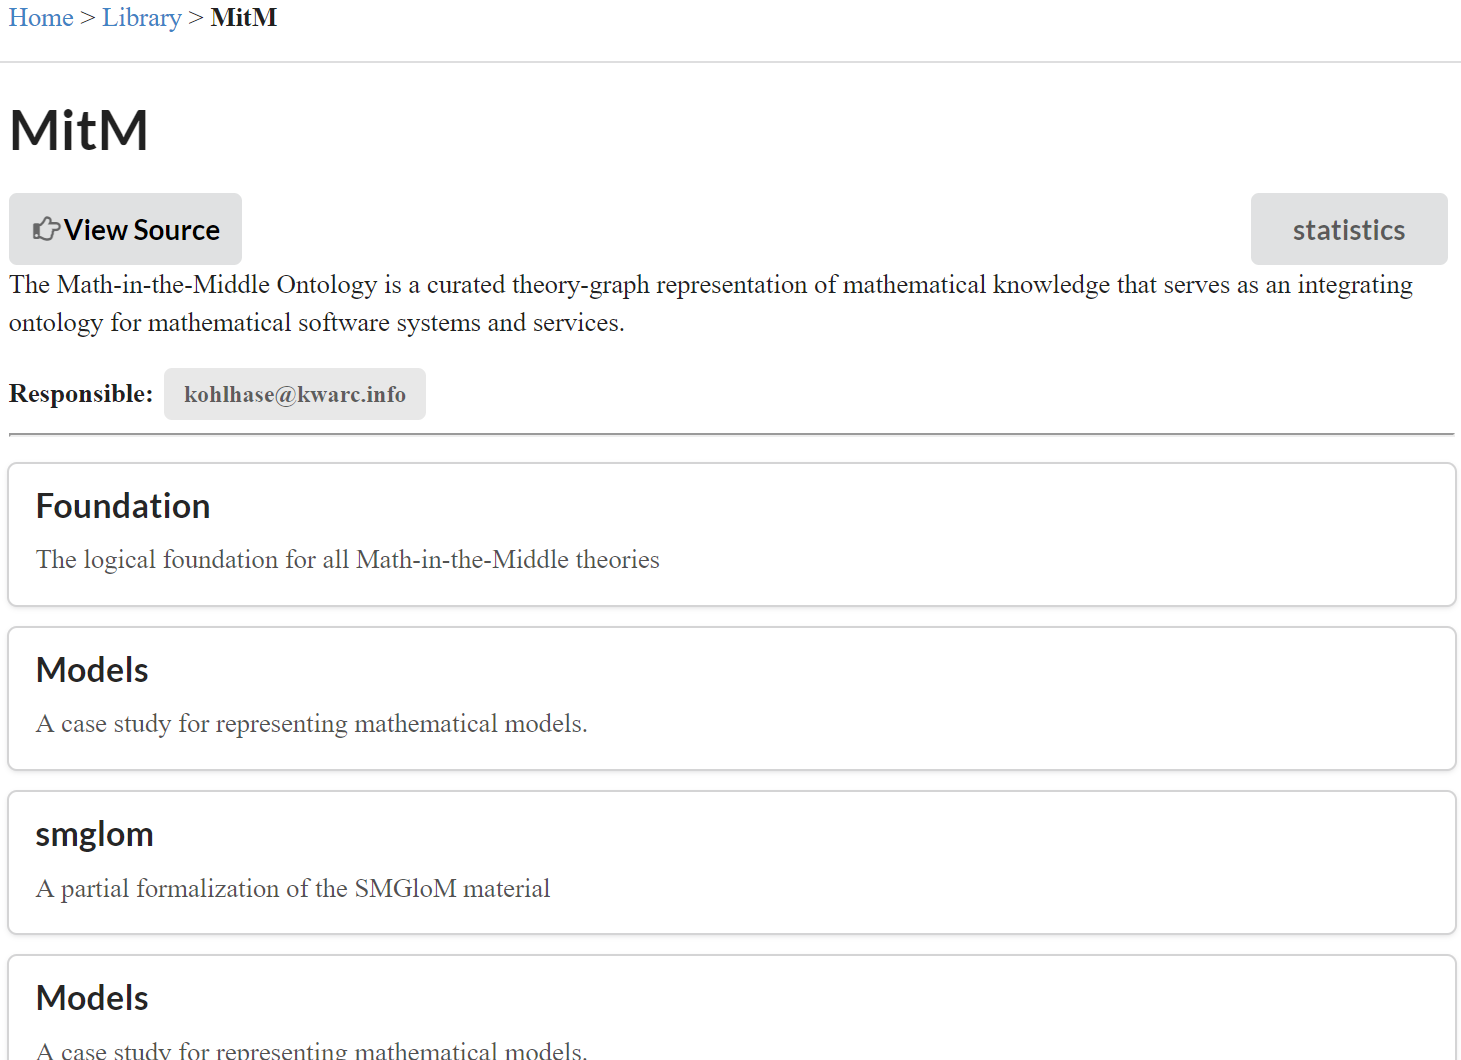
\includegraphics[width=1\textwidth]{group.png}
\caption{a group in the frontend}
\label{fig:group}
\end{figure}
As an example figure \ref{fig:group} shows a screenshot of the MitM group as it is currently depicted on MathHub.info.
Above the numerous archives the group page starts with a header that has the same structure for every group.
It begins with a button that links to its source files on GitLab.
After that follows a description that gives an overview of the groups content.
The header ends with a list of e-mail addresses of the people that maintain the group.

Beneath that there is a list of all the corresponding archives.
Every archive is its own React component that consists of a name and a short teaser that summarizes its content for the user.
By clicking on an entry the user is taken to the corresponding archive-page.

\subsection{Archives}
\begin{figure}[H]
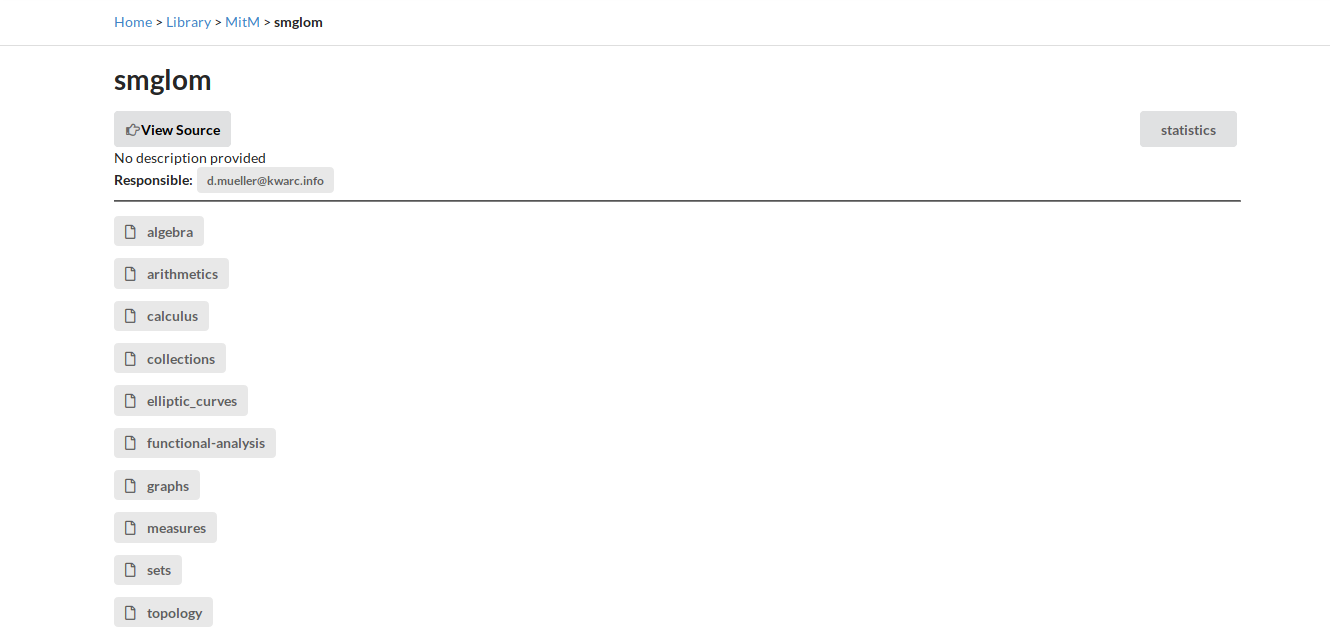
\includegraphics[width=1\textwidth]{archive.png}
\caption{ an archive in the frontend}
\label{fig:archive}
\end{figure}
Figure \ref{fig:archive} shows that the structure of the archive-page is very similar to the group-page.
It also starts with a header that consists of a button that links to the source files, a description of the archive and the e-mail addresses of the responsible people. 

After the header follows a list of the documents in that archive.
There is the main difference between the group-page and the archive page.
The document entries do not have a teaser text so they just link to the document-page.

\subsection{Documents}
\begin{figure}[H]
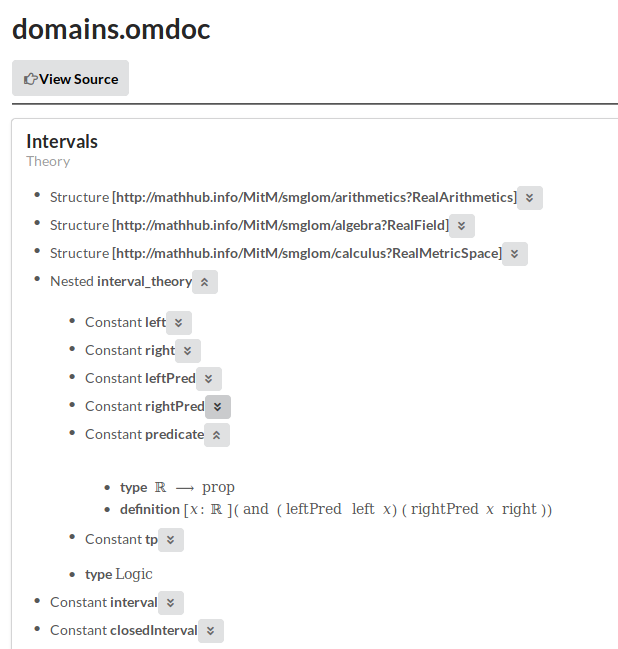
\includegraphics[width=1\textwidth]{document.png}
\caption{a document in the frontend}
\label{fig:doc}
\end{figure}
Depending on the document, the its page can be a combination of modules and opaque elements as well as links to further documents.
Figure \ref{fig:doc} displays a document in the OMDoc format.
There is also a button that links to a documents source file on GitLab\ednote{+ jupyter} if it is in the OMDoc format.

The modules are expandable React components that consist of a name, a type, either theory or view and a button to show further details.
Clicking on the button shows all the declarations and nested theories inside of that module.
These declarations (structure elements, constants, rule constants etc.) and theories can be further extended to show their own content.

In between the modules there can be opaque elements.
These are just text that help the user to understand the content of the document.
So opaque elements make up the informal part of theories in MMT.

\subsection{Statistics}
\begin{figure}[H]
\centerline{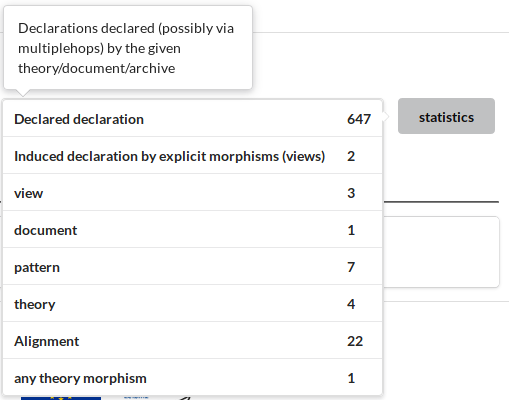
\includegraphics[width=0.6\textwidth]{statistics.png}}
\caption{statistics in the frontend}
\label{fig:stats}
\end{figure}
On every group-, archive- and document-page there also is a statistics button that shows some available statistics about that particular group, archive or document.
When the cursor hovers over a keyword of a statistic that keyword is explained in a pop-up as can be seen in figure \ref{fig:stats}.

\section{The Applications of MathHub} \label{apps}
\subsection{Glossary}
\begin{figure}[H]
\includegraphics[width=1\textwidth]{glossary.png}
\caption{the glossary in the frontend}
\label{fig:glossary}
\end{figure}
As shown in \ref{fig:glossary}, the glossary-page has a tab for every available glossary.
At any given time only the terms are rendered that have an entry in the currently selected language.
Thus there are two possible ways to change languages.
First by changing the language tab of the glossary or second by clicking on a language-button inside an entry.
If such a button with a different language is available, this means this particular entry also exists in that language.

To create a better overview the definition of a term is not immediately shown.
By clicking on an entry its definition becomes visible.

\subsection{Math Dictionary}
\begin{figure}[H]
\includegraphics[width=1\textwidth]{dictionary.png}
\caption{the Math Dictionary in the frontend}
\label{fig:dict}
\end{figure}
Figure \ref{fig:dict} displays the Math Dictionary of MathHub.info.
To translate a term with the help of the Math Dictionary the user has to select the language from a dropdown menu in which the term currently is and also the language to which it should be translated into
Pressing the "translate" - button sends a translation request to the server.
Until the servers responds, the message "translating" is shown and the button is disabled to prevent sending to many translation requests at once.
If a translation exists then the translated term, its definition and potential synonyms are shown and the button is enabled again.
By selecting the same language for "from" and "to" the Math Dictionary can also be used to get the definition for an expression without searching the glossary.

\section{Conclusion} \label{conclusion}
 \ednote{re-iterate everything}
\section{Future Work} \label{future}
Obviously the work on a project like MathHub.info is never completely finished.
There are still many features left that would be a great addition to the frontend to improve the practicality and the overall user experience. \ednote{sounds to trivial?}
The biggest expansions that will be added to MathHub.info in the near future are TGView and MathWebSearch.

\subsection{TGView} 
TGView is a graph viewer with the task to visualize the relations between multiple theories to give a better overview over a system like MathHub.
The distinctive feature of TGView is that its backend sends all necessary data at once so every interaction can be handled by the frontend.
That means that its graphical interface is build on the client side to avoid sending a server request every time the user interacts with the interface, eg move or hide nodes.
Otherwise it would be required to refresh the page on every single change to the graph. 	\cite{tgview}
 
Even though the old MathHub frontend did have static graphs to show the relations between theories, it never integrated TGView.
 
\subsection{MathWebSearch}
Explanation needed!

\subsection{Subset Frontends}
Currently MathHub.info is a place to showcase every MMT group.
But some of these groups could benefit from specialized additional features or a slightly different structure.
So it makes sense to create subset frontends based on MathHub.info.
This way the subset frontends can be designed to perfectly fit their group without taking other groups into account.
In addition to new features they also should have a new Homepage to give the user a more detailed introduction than the short teaser that is shown on MathHub.info.

To summarize, the subset frontends will have a similar makeup as MathHub.info but will be adapted to better represent their content.

\subsection{Issue report: MathHub.info and content}
As of right now there is no direct way for a user to report an issue, a bug or request a new feature.
When this function is integrated into MathHub.info it would be appropriate to distinguish between two different kind of reports.

First, the user should be transferred to GitHub to open a new issue, if they have a problem with the frontend.

Second, if the user finds an issue within the content that is displayed on MathHub.info, they should be redirected to the corresponding GitLab page. 
\subsection{Jupyter Integration}

\printbibliography
\ednote{use this: github.com/KWARC/bibs/kwarc.bib}
\end{document}